\documentclass[12pt,a4paper]{article}
%\documentclass[12pt,twoside,a4paper]{article} %Duplex udskrivning
\usepackage[ansinew]{inputenc}			% Windows

\usepackage[T1]{fontenc} 
\usepackage[danish]{babel}				% Dansk ordbog
\usepackage{amsmath, amsfonts, amssymb} % Matematiske pakker
\usepackage{graphicx} 					% Grafiksk pakke

\usepackage[left	=3cm,
			right	=2cm,
			top		=2.2cm,
			bottom	=2cm
		]{geometry} 					% Sidejustering

%Mellemrum mellem linjerne
\usepackage{setspace}
\setstretch{1.5} %Afstanden
\usepackage{float}

% Links
\usepackage{hyperref}
\hypersetup{ 
	colorlinks	= true, 	% false: boxed links; true: colored links
    urlcolor	= blue,		% color of external links
    linkcolor	= black, 	% color of page numbers
}

% Figur der st�r vilk�rligt
\usepackage{wrapfig}
%\begin{wrapfigure}{r}{0.6\textwidth}
%   \vspace{-20pt}
%	\centering
%	\includegraphics[scale=0.25]{...}
%    \vspace{-20pt}
%    \caption{...}
%  \label{fig:...}
%  \vspace{-10pt}
%\end{wrapfigure}

\usepackage{lastpage}

% Sideops�tning
\usepackage{fancyhdr}					% Header-style
\pagestyle{fancy}
\fancyhf{} % slet alt
\fancyfoot[C]{Side \thepage \text{ af} \pageref{LastPage}} % sidetallet yderst
\lhead[]{\leftmark} % lige side, kapitel titel
\headheight = 35pt
\textheight = 680pt
\footskip 	= 40pt

\renewcommand{\headrulewidth}{0.4pt}
\renewcommand{\footrulewidth}{0.4pt}

\usepackage{enumerate}

\usepackage{subfiles}

%----------------------------------------------------------
% F�lgende er til tabeller
%----------------------------------------------------------
\usepackage{booktabs, cellspace} 		
\addtolength\cellspacetoplimit{10pt}
\addtolength\cellspacebottomlimit{10pt}

%----------------------------------------------------------
% F�lgende er til koder.
% Inds�ttes mellem \begin{lstlisting} og \end{lstlisting}
%----------------------------------------------------------
\usepackage{listings}
\usepackage{color}
\usepackage{textcomp}
\definecolor{listinggray}{gray}{0.9}
\definecolor{lbcolor}{rgb}{0.9,0.9,0.9}
\lstset{
	language		= [Sharp]C,
	keywordstyle	= \bfseries\ttfamily\color[rgb]{0,0,1},
	identifierstyle	= \ttfamily,
	commentstyle	= \color[rgb]{0.133,0.545,0.133},
	stringstyle		= \ttfamily\color[rgb]{0.627,0.126,0.941},
	showstringspaces= false,
	basicstyle		= \small,
	numberstyle		= \footnotesize,
	numbers			= left, % Tal? Udkommenter hvis ikke
	stepnumber		= 1,
	numbersep		= 5pt,
	tabsize			= 2,
	breaklines		= true,
	prebreak 		= \raisebox{0ex}[0ex][0ex]{\ensuremath{\hookleftarrow}},
	breakatwhitespace= false,
	aboveskip		= {1.5\baselineskip},
  	columns			= fixed,
  	upquote			= true,
  	extendedchars	= true,
	lineskip		= 1.5pt,
    xleftmargin		= 17pt,
	framexleftmargin= 17pt,
	framexrightmargin	= 5pt,
	framexbottommargin	= 4pt,
% frame=single,
 	backgroundcolor=\color{lbcolor},
}
\renewcommand*{\lstlistingname}{Kodeudsnit}

\usepackage{caption}
\DeclareCaptionFont{white}{\color{white}}
\DeclareCaptionFormat{listing}{\colorbox[cmyk]{0.43, 0.35, 0.35,0.01}{\parbox{\textwidth}{\hspace{15pt}#1#2#3}}}
\captionsetup[lstlisting]{format=listing,labelfont=white,textfont=white, singlelinecheck=false, margin=0pt, font={bf,footnotesize}}


%----------------------------------------------------------
% F�lgende er tabel over Use Cases - Akt�rer - Forventet 
% 	resultat og checkbox
% Inds�ttes med \begin{testcase} og \end{testcase}
%----------------------------------------------------------
%\usepackage{enumitem,calc}

\newenvironment{testcase}[1]
{
\begin{tabular}{| p{1.2cm} | p{6cm} | p{5.5cm} | l|}\hline
\textbf{TRIN} & \textbf{Aktion / Input} & \textbf{Forventet resultat} & \textbf{CHK} \\
\hline
}
{&\\\hline
\end{tabular}
\\\\
\\\\}
\newcommand\punkt{&\\\hline} 
\newcommand\Aktion{&}
\newcommand\Forventet{&}

%Grader tegn
\newcommand{\degree}{\ensuremath{^\circ}}	% Alle_indstillinger_for_dokumentet
\begin{document}

\begin{center}
 \section*{Simulator manual}
\end{center}

\noindent
Dette dokument beskriver hvordan simulatoren bruges. Efter hvert billede, vil funktionaliteten ved nummeret beskrives.

\begin{figure}[H]
\centering
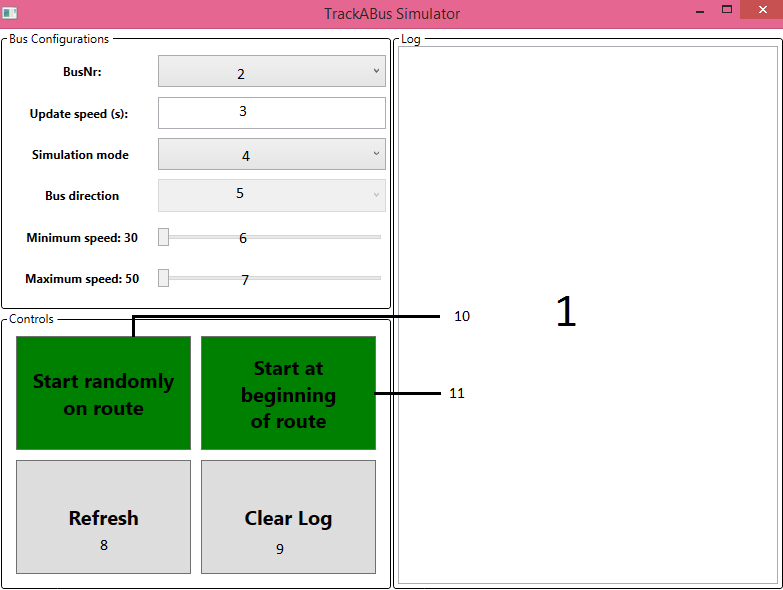
\includegraphics[scale=0.40]{Simulator/Billeder/SimulatorViewStart.png}
\caption{Startsiden for administrator hjemmesiden}
\label{fig:MainScreen}
\end{figure}

\noindent
P� figur \ref{fig:MainScreen} kan simulator sk�rmen ses. Denne sk�rm er den eneste der kan forekomme under simulering.
\begin{enumerate}
	\item Log vindue.
	\begin{itemize}
		\item Alle n�dvendige system beskeder vil vises her, som de forekommer i systemet.
	\end{itemize}		
	\item Rutenummer boks.
	\begin{itemize}
		\item Her kan en rute v�lges, fra en liste af alle ruter som har busser knyttet til sig. En rute skal v�re valgt f�r simulering kan p�begyndes, men hvis det v�lges at simulere alle ruter har denne v�rdi ingen effekt.
	\end{itemize}
	\item Opdateringshastighed
	\begin{itemize}
		\item Tallet beskriver hvor hurtigt de simulerede busser opdaterer. Tallet skal v�re i hele sekunder, og ikke under 1.
	\end{itemize}
		\item Simulerings metoden.
	\begin{itemize}
		\item Beskriver m�den der simuleres. Der kan v�lges at simulere �n bus p� valgt rute, alle busser p� valgt rute og alle busser p� alle ruter. 
	\end{itemize}
		\item Retningen bussen k�rer.
	\begin{itemize}
		\item Her v�lges der hvilken retning de simulerede busser skal k�re. Her kan en specifik retning eller en tilf�ldig retning v�lges. Hvis der kun simuleres �n bus, er det kun den ene bus det g�lder for. Hvis samtlige busser p� ruten simuleres er valget g�ldende for samtlige busser p� ruten, og hvis alle busser i systemet simuleres, vil valgtet v�re g�ldende for alle busser der k�rer p� den valgte rute, og alle andre busser vil k�re i tilf�ldig retning.
	\end{itemize}
	\item Minimums hastigheden.
	\begin{itemize}
		\item Definerer minimums hastigheden for de simulerede busser. Denne kan �ndres p� runtime, men vil altid v�re mindre end, eller lig med maksimums hastigheden. Ved en ny opdatering, vil de simulerede bussers hastighed randomiseres mellem minimum og maksimums hastigheden.
	\end{itemize}
	\item Maksimums hastigheden.
	\begin{itemize}
		\item Definerer maksimums hastigheden for de simulerede busser. Denne kan �ndres p� runtime, men vil altid v�re st�rre end eller ligmed minimums hastigheden. Ved en ny opdatering, vil de simulerede bussers hastighed randomiseres mellem minimum og maksimums hastigheden.
	\end{itemize}
	\item Refresh knap.
	\begin{itemize}
		\item I tilf�lde af, at nye busser er blevet tilf�jet til systemet, mens simulatoren har v�ret k�rt, kan denne knap trykkes, hvorefter listen af mulige ruter genskabes
	\end{itemize}
	\item Clear log knap.
	\begin{itemize}
		\item Fjerner alle indl�g i loggingvinduet.
	\end{itemize}
	\item Start randomly knap.
	\begin{itemize}
		\item Starter simuleringen. Denne knap vil randomisere de simulerede bussers start position p� ruten.
	\end{itemize}
	\item Start at beginning knap.
	\begin{itemize}
		\item Starter simuleringen. Denne knap vil tvinge alle simulerede busser til at starte ved f�rste endestation, som v�lges alt efter hvilken retning, der er blevet defineret.
	\end{itemize}
\end{enumerate}
\end{document}
